\chapter{Experimento}
\label{experimento}

Nesta Seção é apresentado o experimento de implementação de uma RSSF em um ambiente de \emph{Smart Building}, utilizando a implementação do padrão IEEE 802.15.4g SUN dos dispositivos OpenMote-B \cite{tuset2020dataset}. A finalidade deste experimento é avaliar o desempenho da rede analisando valores de PDR e RSSI obtidos.

O experimento foi realizado em um dos prédios do campus Campina Grande do IFPB, Instituto Federal de Educação, Ciência e Tecnologia da Paraíba. O prédio é constituído, principalmente, de salas de escritório e de alguns laboratórios, possuindo 4 andares separados por pisos de concreto. Além desse cenário ser particularmente desafiador para um enlace sem fio, pois, não é possível ter uma linha de visada entre o transmissor e o receptor, e as paredes e pisos facilitam a ocorrência de propagação por múltiplos caminhos, com possibilidade de áreas de sombreamento de sinais.

\section{Visão Geral}
\label{subsec:visaogeral}
A rede é composta por 11 dispositivos transmissores, denominados no restante do texto de Tx, que enviam nove réplicas de mensagens, três para cada modulação do padrão IEEE 802.15.4g SUN. Três receptores, chamados no restante do texto de Rx, foram configurados para receber mensagens em apenas uma das modulações do padrão. Os dispositivos Rx enviam as mensagens recebidas via rádio por uma porta serial para um computador que utiliza um sistema operacional de base GNU/Linux, o Linux Mint 19 e executa um \emph{script Python} que lê as mensagens seriais enviadas pelos dispositivos Rx, estrutura e persiste os dados em um banco de dados InfluxDB. Na Figura \ref{fig:rede_visão_geral} é representada uma visão geral do funcionamento da rede.

\begin{figure}[h]
  \begin{center}
    \caption{Visão Geral da Rede.}
    \includegraphics[width=0.8\textwidth]{./sections/textual/chapters/images/rede_visão_geral.png}\\
    Fonte autoral.
    \label{fig:rede_visão_geral}
  \end{center}
\end{figure}

Os dispositivos Tx foram posicionados nos quatro andares do prédio, em canaletas, como demonstrado na Figura \ref{fig:tx_canaleta}, e no interior de uma sala. Os dispositivos Rx foram colocados no interior do laboratório do GComPI, presente no primeiro piso do prédio.

\begin{figure}[h]
  \begin{center}
    \caption{Exemplo de Posicionamento dos Dispositivos Tx.}
    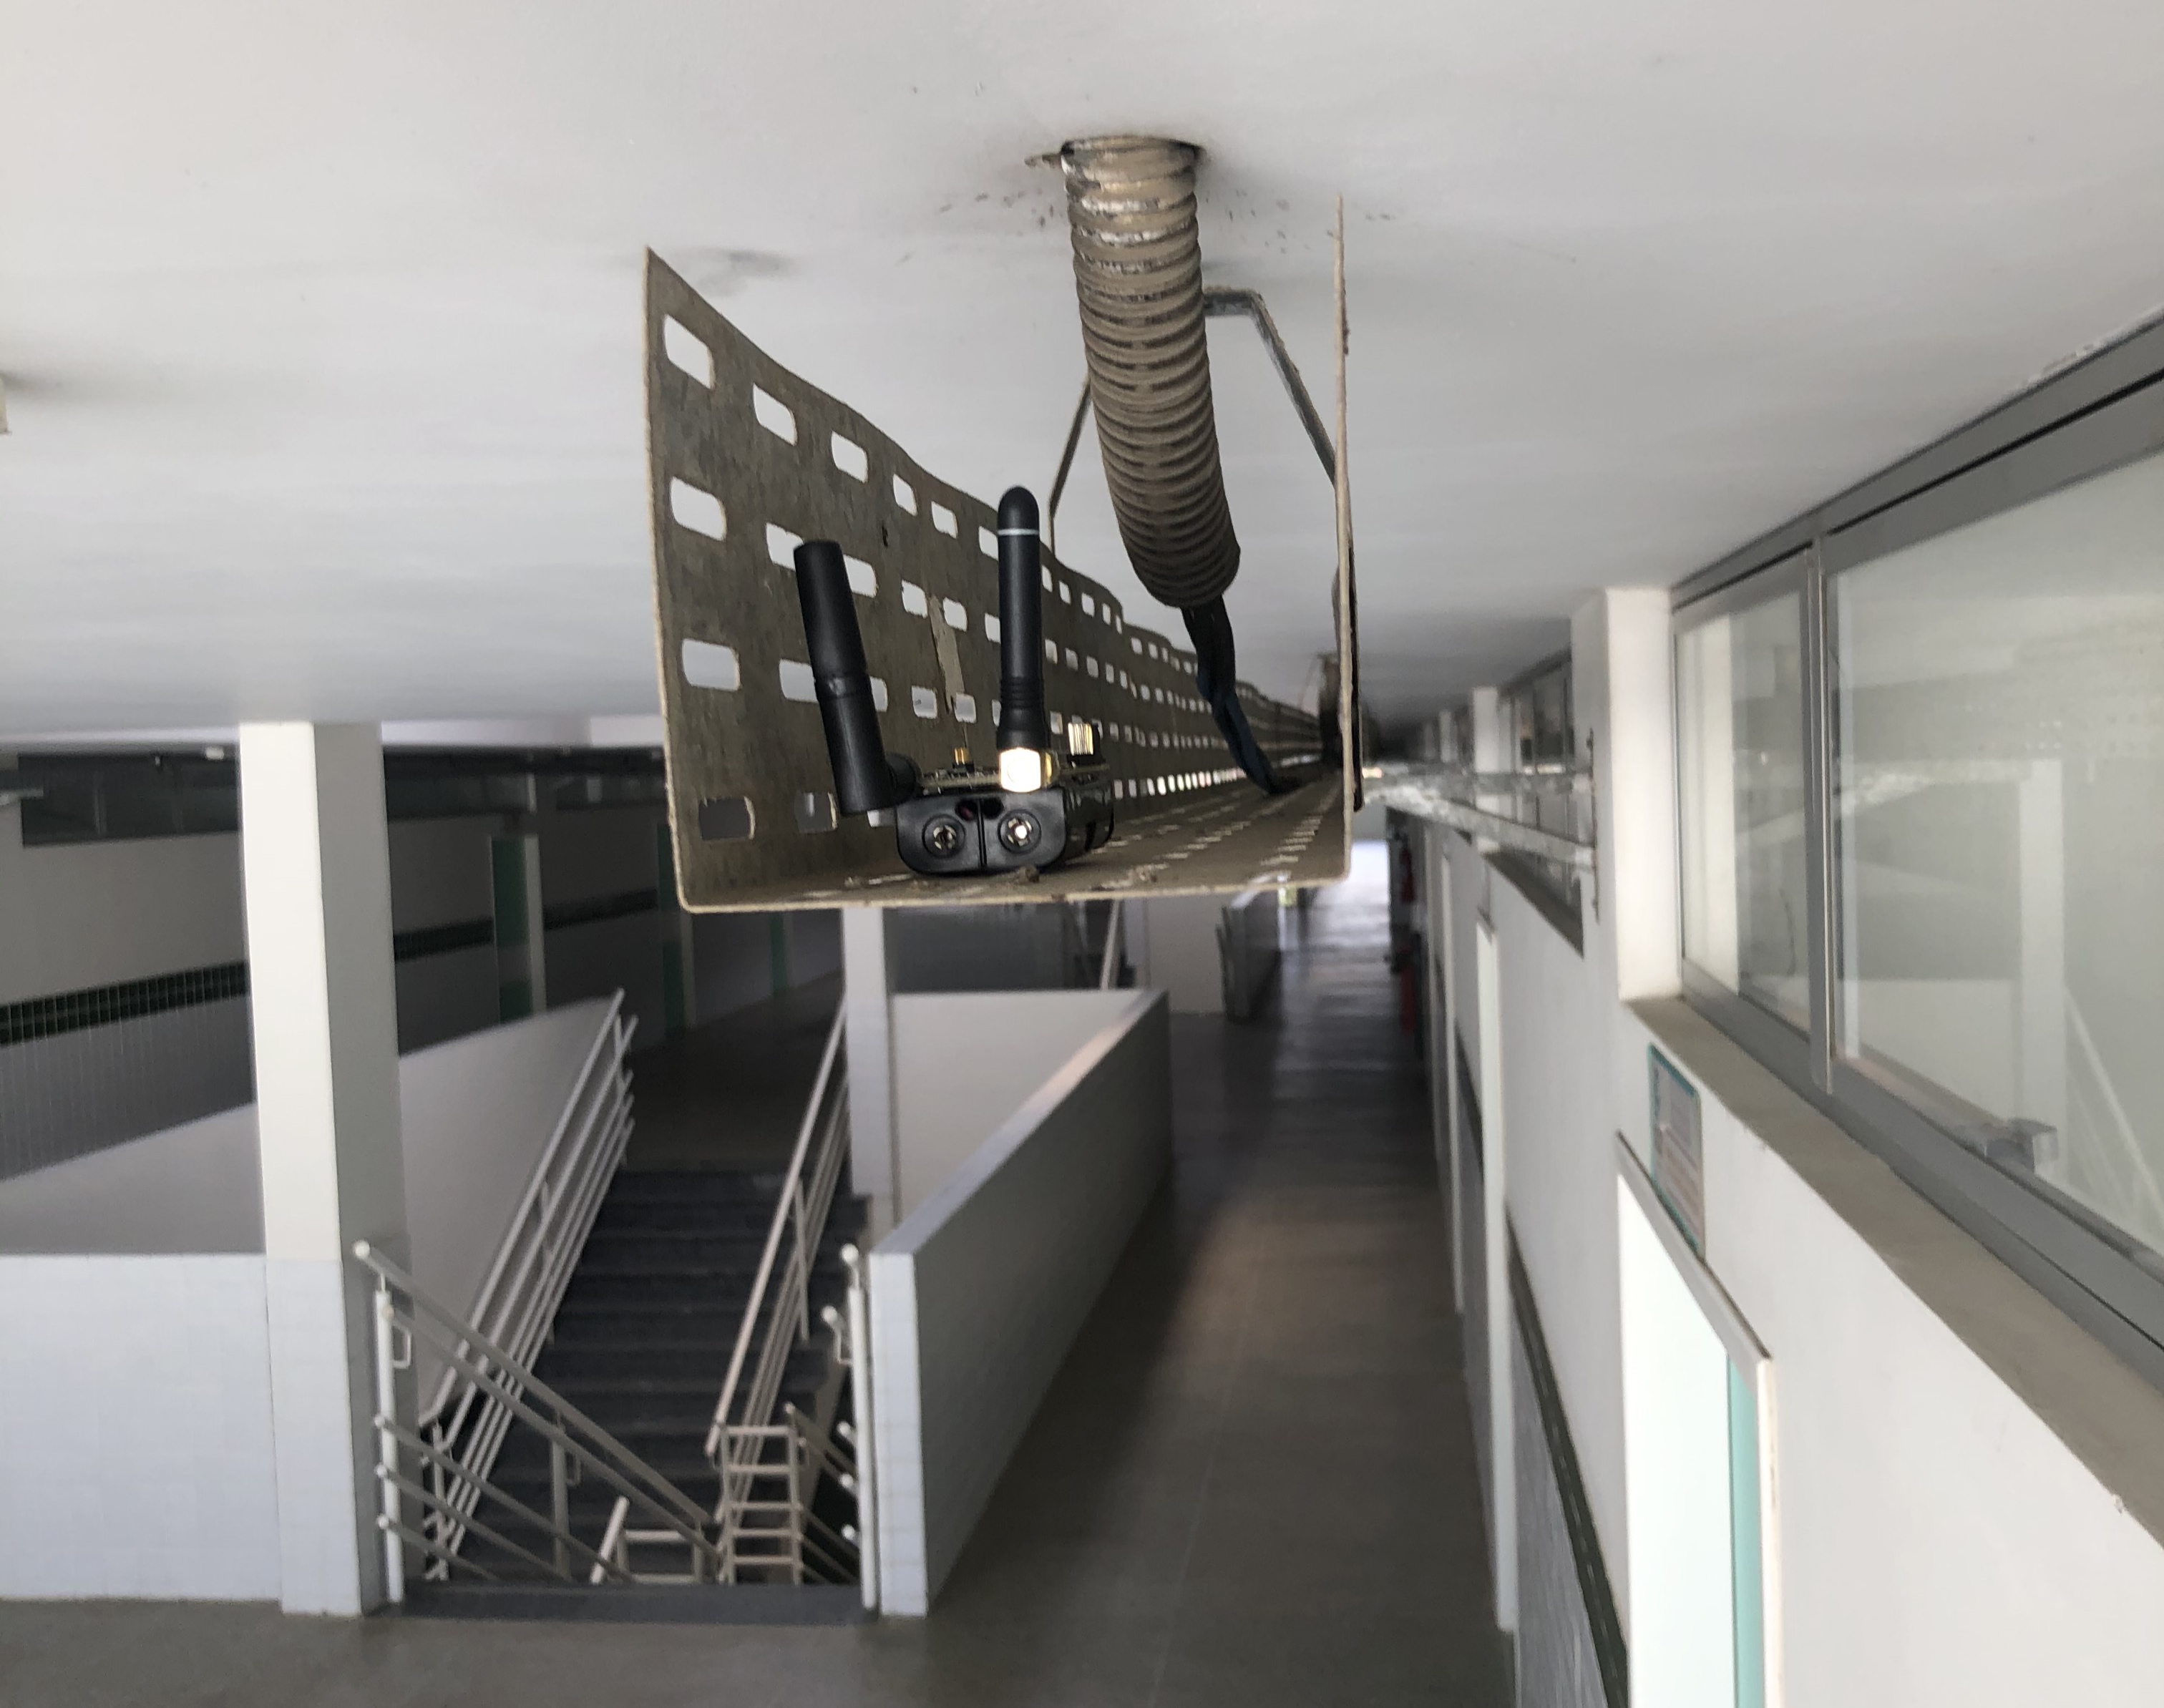
\includegraphics[width=10cm]{./sections/textual/chapters/images/tx_canaleta.jpg}\\
    Fonte autoral.
    \label{fig:tx_canaleta}
  \end{center}
\end{figure}

\section{OpenMote B}
O OpenMote B é um \emph{hardware} de desenvolvimento e prototipação de plataformas IoT. Contém o processador SoC, \emph{System-on-Chip} (Sistema em um \emph{Chip}), CC2535 da Texas Instruments, constituído de um ARM Cortex-M3, com 32 k\emph{bytes} de memoria RAM e 512 k\emph{bytes} de memoria Flash. Embarcado nesse processador, há um transceptor com suporte ao padrão IEEE 802.15.4 que utiliza a modulação DSSS-OQPSK na faixa ISM de 2,4~GHz. O OpenMote B também contém um transceptor AT86RF215 da ATMEL que implementa as três modulações do padrão IEEE 802.15.4g, nas faixas de frequência ISM abaixo de 1~GHz e na faixa ISM de 2,4~GHz \cite{openmoteb-userguide}.

O código-fonte do \emph{firmware} dos dispositivos está presente no repositório em \cite{openmoteb-firmware}. Nele foram realizadas alterações que estão disponíveis no repositório em \cite{openmoteb-gcompi}.

\section{Transmissão dos dados}
Os dispositivos foram configurados para realizar, a cada minuto, três ciclos de envio de mensagens, como representado na Figura \ref{fig:ciclo_envio}. Em cada ciclo são transmitidas três mensagens, uma para cada modulação do padrão. A cada envio de mensagem, o dispositivo pausa por 50 ms. Entre cada ciclo de envio o dispositivo pausa por 100 ms, do primeiro para o segundo ciclo, e 200 ms, do segundo para o terceiro ciclo. Ao realizar os três ciclos de transmissão, o dispositivo entra em modo de espera por 58250 ms totalizando assim 60 segundos para o envio de nove mensagens, cada transmissão, com uma carga útil de 32 \emph{bytes}, leva um total de 100 ms, para a taxa de transmissão de 50 k\emph{bit}/s.

\begin{figure}[h]
  \centering
  \caption{Ciclo de Envio de Mensagens.}
  
\includegraphics[width=\textwidth]{./sections/textual/chapters/images/metodo_ciclo_envio.png}\\
  Fonte autoral.
  \label{fig:ciclo_envio}
\end{figure}

Cada mensagem transmitida é constituída dos seguintes campos:
\begin{itemize}
  \label{table:estruturaTx}
  \item Identificador do dispositivo: um campo de 6 \emph{bytes} que registra um carácter entre ``a'' e ``k'', que identifica cada um dos onze dispositivos Tx;
  \item Identificador de pacote: um campo de 8 \emph{bytes} que registra um contador que é também a identificação do pacote;
  \item Identificador da modulação: um campo de 1 \emph{byte} que registra em qual modulação o pacote foi enviado;
  \item Identificador de Pacote do Transmissor: um campo de 1 \emph{byte} que registra em qual dos ciclos de transmissão (ciclo um, dois ou três) o pacote foi enviado;
  \item Quantidade de Tentativas do CSMA: um campo de 1 \emph{byte} que registra quantas vezes o transmissor sensoriou o canal de radiofrequência antes de realizar a transmissão, o valor pode ser de 1 até 3, caso chegue na terceira tentativa o dispositivo não realiza a transmissão;
  \item Valor de RSSI do transmissor: um campo de 1 \emph{byte} que registra o valor de energia do canal. Se o valor estiver acima do valor apresentado no campo ``Limiar do CCA'' na Tabela \ref{table:config}, o dispositivo espera um tempo aleatório, em milissegundos, e realiza outra tentativa de transmissão.
\end{itemize}

Para completar os 32 \emph{bytes} de carga útil cada mensagem foi preenchida com 14 \emph{bytes}.

% \begin{table}[h!]
%     \centering
%     \begin{tabular}{|c c c c|}
%         \hline
%         Valor       & slug & \makecell{Tamanho   \\ (\emph{bytes})} & Descrição                                                                                \\ [0.5ex]
%         \hline\hline
%         \makecell{Identificador                  \\ do dispositivo}           &      & 6                                          & Uma letra entre ``a'' e ``k''                                                            \\\hline
%         \makecell{Identificador                  \\ de pacote}                &      & 8                                          & Um número inteiro positivo                                                               \\\hline
%         \makecell{Identificador                  \\ da modulação}             &      & 1                                          & O número 1, 2 ou 3\footnote{Respectivamente as modulações SUN-FSK, SUN-OQPSK e SUN-OFDM} \\\hline
%         \makecell{Identificador                  \\ de Pacote do Transmissor} &      & 1                                          & \makecell{Em qual ciclo de envio foi transmitido\\(ciclo 1, 2 ou 3)}\\\hline
%         \makecell{Quantidade de                  \\ Tentativas do CSMA}       &      & 1                                          & \makecell{Número de tentativas do CSMA\\(máximo de 3 tentativas)}                                                \\\hline
%         \makecell{Valor de RSSI                  \\ do transmissor}           &      & 1                                          & \makecell{Quantidade de energia registrada\\no momento da transmissão}                                                                                        \\\hline
%         \makecell{} &      &                   & \\\hline                                                                                        \\ \hline
%         \hline
%     \end{tabular}
%     \caption{Configurações utilizadas de cada modulação.}
%     \label{table:estruturaTx}
% \end{table}

Na Tabela \ref{table:config} estão descritas as configurações de operação de cada modulação.
\begin{table}[h!]
  \centering
  \begin{tabular}{|c c c c|}
    \hline
    Modulação & SUN-FSK & SUN-OQPSK & SUN-OFDM \\ [0.5ex]
    \hline\hline
    \makecell{Taxa de                          \\transmissão(K\emph{bit}/s)    } & 50      & 50                       & 50       \\\hline
    \makecell{Tipo de                          \\Modulação                     } & BFSK    & OQPSK                    & BPSK     \\\hline
    \makecell{Índice de                        \\Modulação                   } & 1.0     & N/A                      & N/A      \\\hline
    \makecell{Taxa de \emph{Chips}             \\(k\emph{chips}/s) } &   N/A      & 100                      & N/A      \\\hline
    \makecell{Modo de                          \\Espalhamento                  } & N/A     & \makecell{SHR:(32,1)-DSS            \\ PHR:(8,1)-DSS\\ PSDU:none} & N/A      \\\hline
    \makecell{Frequência                       \\Central (MHz)              } & 902,2   & 904                      & 902,8    \\\hline
    \makecell{Largura de                       \\banda do canal                                                               \\(MHz)        } & 0,2     & 2                     & 0,8      \\\hline
    \makecell{Canais                           \\disponíveis                    } & 129     & 12                       & 31       \\\hline
    \makecell{Potência de                      \\Transmissão (dBm)         } & 15      & 15                       & 9        \\\hline
    \makecell{Sensibilidade de                 \\Recepção (dBm)       } & -114    & -116                     & -111     \\\hline
    \makecell{Limiar do CCA                    \\(dBm)                   } & -94     & -93                      & -91      \\ \hline
    \hline
  \end{tabular}
  \caption{Configurações utilizadas de cada modulação.}
  \label{table:config}
\end{table}


\section{Recepção e Persistência dos dados}
Os dispositivos Rx foram configurados para, a cada sinal recebido, verificar o valor de RSSI da transmissão e concatenar este valor na sequência de bytes recebida. A sequência é envelopada utilizando o protocolo HDLC, \emph{High-Level Data Link Control} (Controle de Enlace de Dados de Alto Nível, em tradução livre), este protocolo torna a transmissão serial mais robusta e facilita a leitura dos dados na serial no receptor \cite{tanembaum2011}. Então, essa sequência é transmitida pela porta serial para o computador no qual os dispositivos Rx estão conectados.

No computador conectado, as mensagens recebidas são processadas por  meio de um \emph{script Python}. Cada mensagem recebida é extraída do envelope HDLC e se não ocorrer problemas, os \emph{bytes} da mensagem são lidos e armazenados numa estrutura chave-valor da linguagem \emph{Python}, chamada dicionário. Cada chave é um dos campos citados na Seção \ref{table:estruturaTx} e o RSSI adicionado pelo dispositivo Rx. Nessa estrutura são adicionados alguns valores de controle, por exemplo, a quantidade de pacotes seriais recebidos e extraídos corretamente pelo HDLC, e alguns campos relativos ao banco de dados, como a Tabela em que os dados serão armazenados.

Com todos os dados estruturados em um dicionário, eles são enviados utilizando uma biblioteca de funções que facilita a comunicação com o banco de dados, para o qual é utilizada uma função para enviar os dados estruturados. Foi utilizado o InfluxDB, um banco de dados não-relacional de séries temporais otimizado para armazenar dados com marcas temporais, ou seja, os dados armazenados estão relacionados a um intervalo específico \cite{influxData}.

O código do \emph{script Python} está disponível no repositório \cite{openmoteb-serialReader}.

% \begin{lstlisting}[language=Python,tabsize=2]
%     data = [
%     {
%         "measurement": "transmissionData",
%         "tags": {
%             "deviceID": chr(deviceID[0])
%         },
%         "fields":{
%             "counter":     counter,
%             "txMode":      txMode,
%             "txCounter":   txCounter,
%             "csmaRetries": csmaRetries,
%             "csmaRSSI":    csmaRSSI,
%             "rssi":        rssi
%         }
% }
% \end{lstlisting}

